\documentclass{article}
\usepackage{graphicx} % Required for inserting images
\usepackage{amssymb}
\usepackage{amsmath}
\usepackage{amsfonts}
%\usepackage{extarrows}
\usepackage{soul}
\tolerance=1
\emergencystretch=\maxdimen
\hyphenpenalty=10000
\hbadness=10000
\let\oldemptyset\emptyset
\usepackage[T1]{fontenc}

\author{Amnézic}
\date{}
\title{Modèle OSI}

\begin{document}
\maketitle
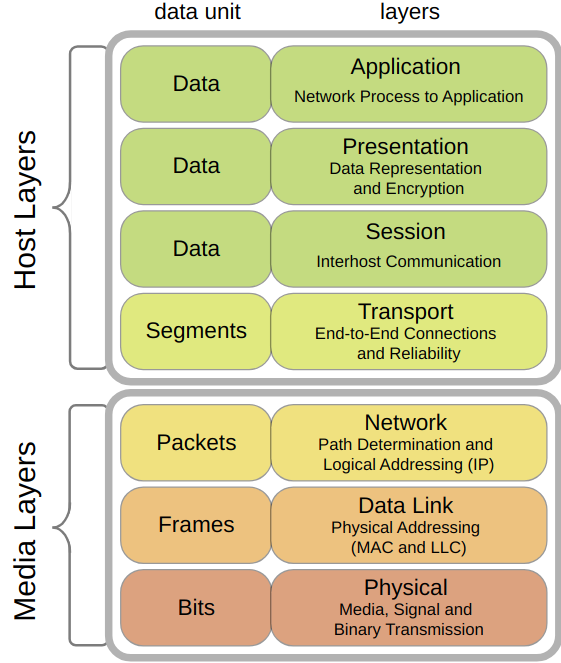
\includegraphics[scale=0.5]{OSI_model.png}
\newpage
\tableofcontents
\newpage

\section{Introduction}
Le modèle d'Interconnexion des Systèmes Ouverts (\textit{Open Systems Interconnection model} en anglais) est un modèle conceptuel de l'ISO qui permet d'obtenir une base commune pour la coordination des standards dans le développement des systèmes internconnectés. Ce modèle est constitué de sept niveaux que nous développerons par la suite. En clair, ce modèle permet de découper un système de comunication en plusieurs parties afin de mieux les comprendre et les mettre en place. Ce modèle est un incoutournable dans le domaine du développement de logiciels car il est la base de chaque projet software. Il permet mettre en place des règles pour la communications entre ordinateurs, du bit jusqu'aux paquets de données. Le texte de la norme proprement dite est très abstrait car il se veut applicable à de nombreux types de réseaux.
Il est important de comprendre que le modèle OSI crée des normes afin de faciliter les communications entre machines mais ne définit pas de protocole précis.

Voici quelques termes qu'il est nécessaire de définir :
\textbf{Définitons}
\begin{itemize}
    \item service : description abstraite de fonctionnalités à l'aide de commandes ou événements telles qu'une demande de connexion ou une réception de données
    \item protocole : ensemble de messages et de règles d'échange réalisant un service
    \item interface : moyen concret d'utiliser le service, càd un ensemble de bibliothèques et de jeux de registres
\end{itemize}

\section{Couche 1 : Physique}
La couche « physique » est chargée de la transmission effective des signaux entre les interlocuteurs. Son service est limité à l'émission et la réception d'un bit ou d'un train (groupe) de bits continu. Concrètement, elle se charge de l'envoi et de la réception de signaux électro-magnétiques. Pour ere plus précis, il décide de la manière dont sont transmises et reçues. La couche physique est constituée de circuits électroniques de diffusion
\section{Couche 2 : Liaison}
\section{Couche 3 : Réseaux}
\section{Couche 4 : Transport}
\section{Couche 5 : Session}
\section{Couche 6 : Présentation}
\section{Couche 7 : Application}


\section{Sujets annexes à regarder :}

\end{document}